\documentclass[11pt]{article}
\usepackage[a4paper,margin=2cm, bottom=2.5cm, top=2cm, headheight=15pt]{geometry}
\usepackage{chemfig}
\usepackage{graphicx}
\usepackage{fancyhdr}
\usepackage[german]{babel}
\usepackage{wrapfig}
\usepackage{url}
\usepackage{array}
\usepackage[T1]{fontenc}

\renewcommand{\footrulewidth}{1pt}

\begin{document}

\pagestyle{fancy}

\fancyhead{}
\fancyhead[L]{Julian Galluzzo, J1 Leistungskurs Chemie 2022/24}
\fancyhead[R]{\textbf{ 20. April 2023}}

\fancyfoot{}
\fancyfoot[L]{\fontfamily{pcr}\selectfont\footnotesize Das Haber-Bosch-Verfahren}
\fancyfoot[r]{\fontfamily{pcr}\selectfont\footnotesize ...\jobname.tex}

\section*{\LARGE{Das Haber-Bosch-Verfahren}}
\vspace{.5cm}
\subsection*{Die Bedeutsamkeit des Stickstoffs}

    \begin{itemize}
        \item Stickstoff ist ein wichtiger Bestandteil aller Lebewesen:
        \begin{itemize}
            \item[$\rightarrow$] Proteine (wichtiger Bestandteil der Aminosäuren)
            \item[$\rightarrow$] bei Pflanzen, z.B. Chlorophyll
            \item[$\rightarrow$] Nukleinsäuren (DNA und RNA)
        \end{itemize}
        \item ebenfalls für Sprengstoffe eingesetzt, z.B. bei Kalium- und Natriumnitrat
    \end{itemize} 
\section*{Das Verfahren}
Für die Ammoniaksynthese müssen Stickstoff und Wasserstoff zusammen reagieren. 
$$N_{2(g)}\hspace{.15cm} +\hspace{.15cm} 3H_{2(g)}\hspace{.25cm} \rightleftharpoons\hspace{.25cm} 2NH_{3(g)}\hspace{.5cm}|\hspace{.1cm}exotherm$$
\subsection*{Einflussmöglichkeiten}
    \textbf{Katalysator}
        \begin{itemize}
            \item ein Katalysator wird eingesetzt: Magnetit bzw. Ferrit (Ein Gemisch aus $FeO$ und $Fe_2O_3$)
            \item durch \textbf{Adsorption} der Moleküle an das Ferrit (Anlagerung an der Oberfläche) werden Stickstoff und Wasserstoff leichter gespalten (\textbf{Dissoziation})
            \item Stickstoff und Wasserstoff reagieren schrittweise zu Ammoniak, das schließlich \textbf{desorbiert} (Abtrennung von der Oberfläche)
    \end{itemize}

    \hspace{-.75cm}\begin{tabular}{m{8.5cm} m{8.5cm}} 
        \textbf{Temperatur}
        \begin{itemize}
            \item Reaktion läuft exotherm ab
            \item bei Temperaturerniedrigung wird Produktseite begünstigt
            \item Idealtemperatur für Synthese liegt bei ca. 500°C wegen Katalysator
        \end{itemize}
        &
        \textbf{Druck}
        \begin{itemize}
            \item Auf der Eduktseite befinden sich mehr Teilchen
            \item Durch der Druckerhöhung wird die Produktseite begünstigt
            \item 300 Bar als Idealdruck
        \end{itemize}
        
    \end{tabular}
        
\subsection*{Die industrielle Umsetzung} 
    
        \begin{center}
            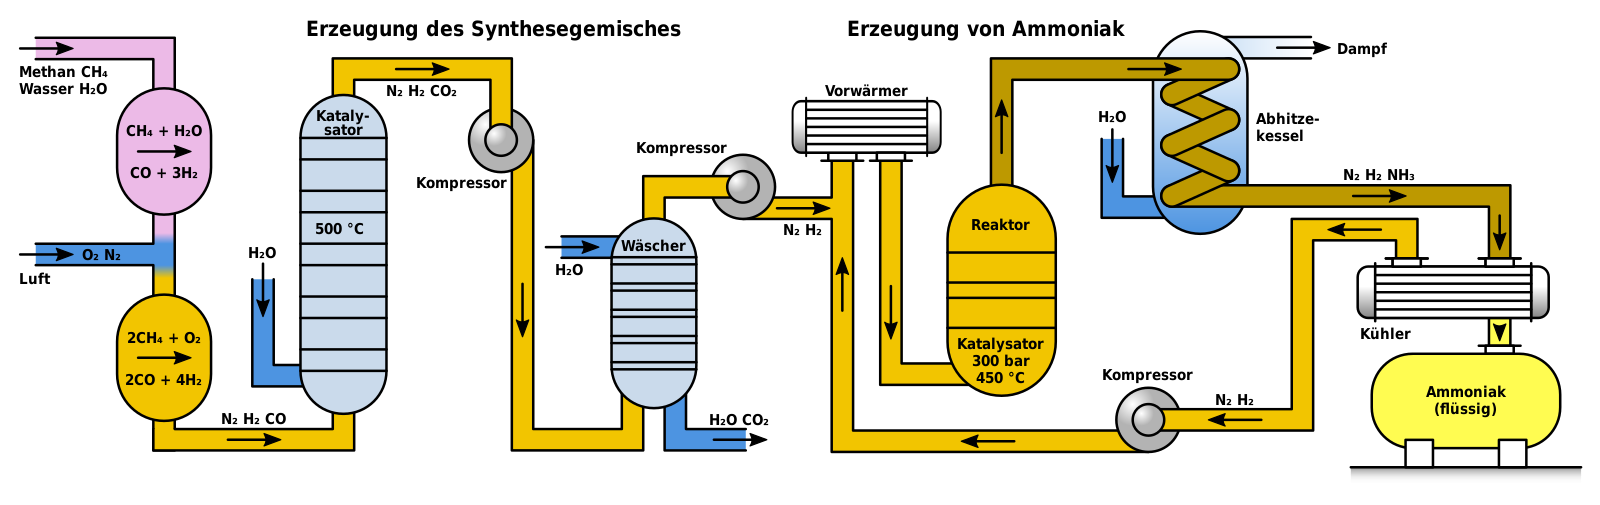
\includegraphics[scale=.31]{Haber-Bosch-Process.png}    
        \end{center}

\subsection*{Fritz Haber}

\begin{itemize}
    \item geboren 1868 in Breslau, Polen; gestorben 1934 in Basel
    \item war auf die synthetische Herstellung on nitratbasierte Sprengstoffe ausgerichtet
    \item durch seine Entdeckung als nationaler Held angesehen
    \begin{itemize}
        \item[$\rightarrow$] wurde Leiter des Kaiser-Wilhelm-Institut in Berlin
        \item[$\rightarrow$] erhielt den Nobelpreis für Chemie in 1918, jedoch war Preisübergabe sehr umstritten
    \end{itemize}
    \item war stark im 1. Weltkrieg beteiligt und für die Herstellung von chemischen Waffen wie Chlor- und Senfgas zuständig
    \item musste nach NS-Übernahme wegen jüdischer Abstammung von der Leitung des Kaiser-Wilhelm-Instituts zurücktreten
\end{itemize}

\subsection*{Carl Bosch}
\begin{itemize}
    \item geboren 1874 in Köln; gestorben 1940 in Heidelberg
    \item Ingenieur bei BASF
    \item brachte das Verfahren auf die industrielle Ebene
    \begin{itemize}
        \item[$\rightarrow$] entwickelte den ersten Teil des Haber-Bosch-Verfahrens für die Erzeugung des Synthesegemisches
    \end{itemize}
    \item spielte eine wichtige Rolle beim Bau der ersten Fabrik in Ludwigshafen-Oppau
\end{itemize}    

\section*{Auswirkungen auf die heutige Welt}
  
        \begin{tabular}{m{7.5cm} | m{8.5cm}} 
            \textbf{Positive Aspekte}
            \begin{itemize}
                \item weniger Länder wurden von der südamerikanischen Guano-Versorgung abhängig
                \item die Erde kann jetzt 4 Milliarden Menschen mehr aufnehmen früher
                \item du könntest sogar dein Leben Habers Erfindung verdanken!
            \end{itemize} 
&
            \textbf{Negative Aspekte}
            \begin{itemize}
                  \item stickstoffbasierte Sprengstoffindustrie ist seit dem Haber-Bosch-Verfahren in Gang gekommen
                  \item Überproduktion: Ammoniak gelangt in Flüssen und Meeren
                \begin{itemize}
                    \item[$\rightarrow$] übermäßige Algenbewachsung, die zum Überverbrauch von Sauerstoff führt (Entstehung von "Dead zones")
                \end{itemize}
            \end{itemize}
        \end{tabular}

\section*{Fazit}
\begin{itemize}
    \item ``Turning air into bread'' - obwohl er Deutschland auf den nächsten Krieg vorbereiten wollte, löste er am Ende eines der größten Probleme seiner Zeit
    \begin{itemize}
        \item[$\rightarrow$] Fritz Haber lässt sich bis heute noch schwierig als Held oder Schurke einordnen
    \end{itemize} 
    \item die Ammoniaksynthese ermöglichte die Herstellung großer Mengen an Munition für die deutsche Armee
    \item eine nachhaltige Alternative für die Herstellung von Ammoniak bzw. des Synthesegemisches ist noch zu finden
    \item der wichtigste Prozess zur Schaffung einer modernen Welt wie wir sie kennen
\end{itemize}

\newpage

\section*{Quellen (Stand: 23. März 2023)}

\small\begin{itemize}
            \item \url{https://www.youtube.com/watch?v=EvknN89JoWo}
            \item \url{https://www.worldatlas.com/articles/what-is-guano.html}
            \item \url{https://www.science.org/content/article/how-bird-poop-helps-cool-arctic}
            \item \url{https://utopia.de/ratgeber/guano-duenger-besonderheiten-anwendung-und-nachteile/} 
            \item \url{https://99percentinvisible.org/episode/guano-mania/}
            \item \url{https://rootsofprogress.org/turning-air-into-bread}
            \item \url{https://www.dhm.de/lemo/biografie/fritz-haber}
            \item \url{https://www.chemie.de/lexikon/Ammoniak.html}
            \item \url{https://www.basf.com/global/de/media/events/2019/full-year-results/photos-pk.fragment.html/overview_copy_copy_c$/global/press-photos/de/photos/2019/02/annual-press-conference/10_5114_Ammonia_plant_at_Ludwigshafen_site.jpg.html}
            \item \url{http://daten.didaktikchemie.uni-bayreuth.de/umat/haber/archiv/haber.htm}
            \item \url{https://historycollection.com/fritz-haber-the-monster-who-made-the-modern-world-possible/}
            \item \url{https://chemicalengineeringworld.com/nfpa-national-fire-protection-association/}
            \item \url{https://www.lgt.tw/science/2018/11/21/lack-of-nitrogen.html}
            \item \url{https://www.nagwa.com/en/videos/590147806076/}
            \item \url{https://www.weforum.org/agenda/2021/12/world-population-history}
            \item \url{https://www.discovermagazine.com/the-sciences/6-times-we-tried-to-extract-gold-from-seawater}
            \item \url{https://www.youtube.com/watch?v=tdEE5uvFhOM}
            \item \url{https://www.wired.com/2015/10/nobel-committee-hasnt-always-picked-right-winners/}
            \item The Alchemy of Air. A Jewish Genius, a Doomed Tycoon, and the Scientific Discovery That Fed the World but Fueled the Rise of Hitler, Thomas Hager
            \item Fokus Chemie · Gesamtband Sekundarstufe II
        \end{itemize}
\end{document}
